\section{Introduction}
\label{sec:introduction}

Speech language models (SLMs) build on established capabilities in speech understanding and generation, as well as earlier research on dialogue interaction~\cite{DBLP:conf/nips/BaevskiZMA20,DBLP:conf/icml/RadfordKXBMS23,DBLP:conf/naacl/RauxE09,DBLP:conf/icassp/ShenPWSJYCZWRSA18}. By integrating these foundations with the reasoning and instruction-following capabilities of large language models (LLMs), recent systems have introduced different ways to process spoken information and organize conversational responses~\cite{DBLP:conf/emnlp/ZhangLZZWZQ23,DBLP:conf/iclr/TangYSC000M024,DBLP:conf/iclr/FangGZMZ025,DBLP:journals/corr/abs-2604-15804}. These approaches range from cascaded pipelines to native speech-to-speech models.~\cite{DBLP:conf/aaai/HuangLYSCYWHHLR24,DBLP:journals/corr/abs-2604-15804,DBLP:journals/corr/abs-2412-02612,DBLP:journals/corr/abs-2410-00037}. Understanding their evolution requires examining how these technical choices shape the way a system participates in conversation.

However, architectural paradigms and interaction capabilities describe related but distinct aspects of this development. An end-to-end speech model can remain turn-based, whereas a modular pipeline can support full-duplex dialogue~\cite{DBLP:conf/emnlp/ZhangLZZWZQ23,DBLP:journals/corr/abs-2412-02612,DBLP:journals/corr/abs-2502-13472,DBLP:journals/corr/abs-2509-06502}. Moreover, systems described as full-duplex may adopt distinct response strategies for conversational events such as interruptions or side-talk.~\cite{DBLP:journals/corr/abs-2410-00037,DBLP:journals/corr/abs-2501-06282,DBLP:conf/icml/WangLFZS000M25,DBLP:conf/acl/ZhangCDCWZLYTDZ25}. Conversely, similar interaction behaviors can also arise from different architectural paradigms~\cite{DBLP:journals/corr/abs-2502-13472,DBLP:journals/corr/abs-2501-06282,DBLP:conf/icml/WangLFZS000M25,DBLP:conf/acl/ZhangCDCWZLYTDZ25}. Architectural paradigms and individual interaction capabilities each provide only a partial view of the field’s development. A more complete account requires examining how different technical routes support different forms of interaction and shape the user’s experience.


% Existing surveys provide complementary accounts of speech language models and full-duplex spoken dialogue systems~\cite{DBLP:conf/acl/CuiYJMZWGK25,DBLP:journals/corr/abs-2411-13577,DBLP:journals/corr/abs-2509-14515,lu2026surveyfullduplexspokendialogue}. Understanding their development as a whole, however, requires connecting advances in individual capabilities to the forms of interaction they support. The role of speech in language modeling and the model's involvement in conversational coordination can vary even among systems with similar architectures, while different implementations may address the same interaction needs. Interaction therefore provides the common basis needed to interpret these intersecting developments. From this perspective, we can connect otherwise dispersed work, explain how different technical choices shape the interaction experience, and trace the capabilities needed as spoken dialogue extends toward broader collaboration.

Existing surveys provide complementary accounts of speech language models and spoken dialogue systems~\cite{DBLP:conf/acl/CuiYJMZWGK25,DBLP:journals/corr/abs-2411-13577,DBLP:journals/corr/abs-2509-14515,lu2026surveyfullduplexspokendialogue}. Understanding these developments as a whole requires examining how technical choices jointly support conversational content and timing. The appropriateness of a contribution depends on both its content and its speaking timing within the exchange, while timing decisions themselves depend on the content and context of the conversation. An interaction perspective therefore provides a common basis for relating different technical routes to the communication requirements they address and for explaining their implications for the user's experience.


In this survey, we revisit the technical paradigms of speech language models from an interaction perspective. We systematically examine the relationships between individual capabilities and intersecting technical routes, explain how different design choices support or constrain the interaction experience, and use this analysis to identify capability requirements for future speech interaction. 
Our roadmap, summarized in Figure~\ref{fig:audio-interaction-roadmap}, begins with speech components as the representational foundation of interaction. We then examine how language is modeled through speech and text in half-duplex interaction,and how the conversational floor is managed in full-duplex interaction.
Across both domains, we organize the subcategories along a spectrum of internalization, from externally orchestrated mechanisms to model-native capabilities. 
This shared principle unifies the two taxonomies, providing a consistent framework for relating architectural choices to interaction capabilities.


\begin{figure}[!t]
    \centering
    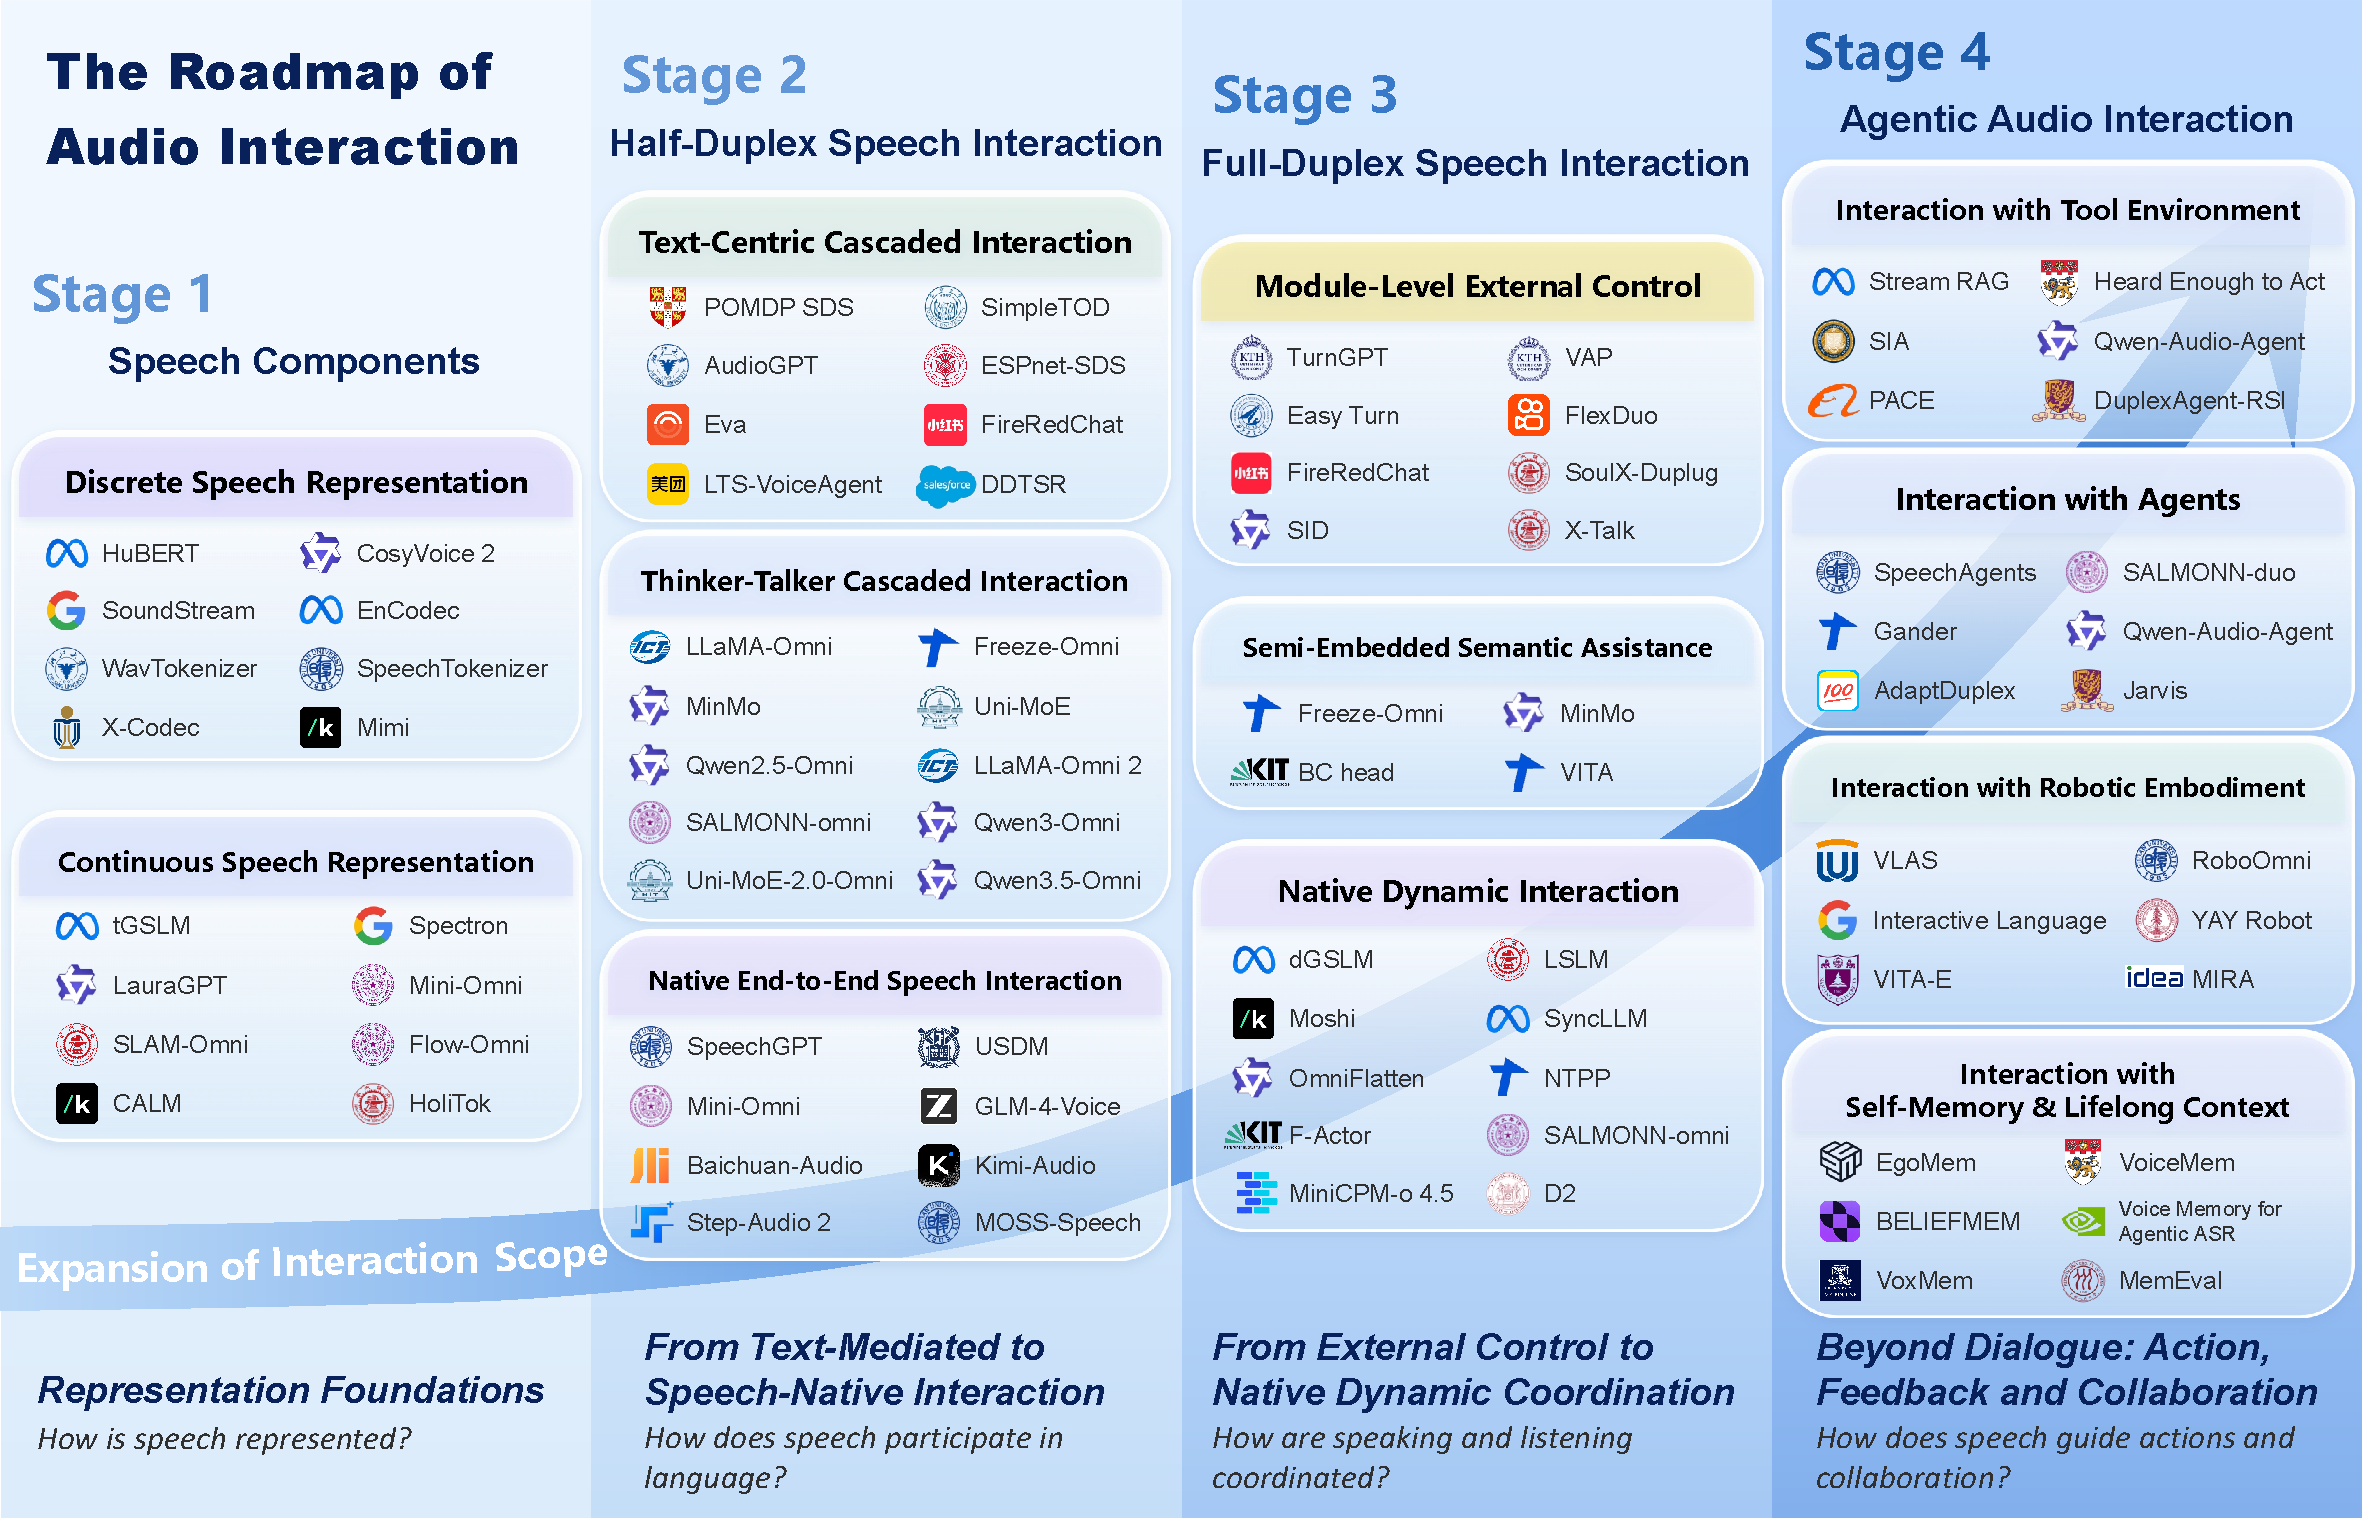
\includegraphics[width=\textwidth,height=0.78\textheight,keepaspectratio]{figures/roadmap_of_audio_interaction.pdf}
    \caption{The roadmap of audio interaction. The vertical arrow traces the expansion in scope from speech representation to language modeling, floor management, and agentic interaction. The horizontal arrow shows increasing internalization in language modeling and floor management.}
    \label{fig:audio-interaction-roadmap}
\end{figure}

Building on this analysis, we consider agentic audio interaction as a forward-looking extension of spoken dialogue. In this outlook, speech provides the primary interface between users and agents, while agents act in digital and physical environments. Existing work on tool use, agent collaboration, robotic embodiment, and persistent memory offers initial foundations for this direction~\cite{DBLP:conf/aaai/HuangLYSCYWHHLR24,DBLP:journals/corr/abs-2401-03945,DBLP:conf/iclr/ZhaoD0GB0W25,DBLP:conf/chi/ZulfikarCM24,DBLP:conf/coling/KirmayrSSMA25}. Through spoken interaction, users can express and refine their goals, while agents communicate the outcomes of their actions and respond to further guidance. The scope of interaction thus expands beyond conversational exchange to encompass actions and environmental feedback, with speech connecting these activities to the user. We examine the capabilities required for speech language models to support this expanded role, distinguishing demonstrated mechanisms from the prospect of sustained collaboration.

% Building on this analysis, we consider agentic audio interaction as a forward-looking extension of spoken dialogue. In this outlook, speech provides the primary interface between users and agents, while agents act in digital and physical environments. Existing work on tool use, agent collaboration, robotic embodiment, and persistent memory offers initial foundations for this direction~\cite{DBLP:conf/aaai/HuangLYSCYWHHLR24,DBLP:journals/corr/abs-2401-03945,DBLP:conf/iclr/ZhaoD0GB0W25,DBLP:conf/chi/ZulfikarCM24,DBLP:conf/coling/KirmayrSSMA25}. Through spoken interaction, users can express and refine their goals, while the system communicates action outcomes and responds to further guidance. We examine how speech interaction models mediate between users' evolving needs and agents' execution capabilities, maintaining continuity between dialogue, action, and feedback.

To complement our analysis of technical approaches, we review training datasets and evaluation benchmarks for speech interaction. We organize these resources around conversational content and timing, reflecting our view that the interaction experience depends on their coordination. The two dimensions cut across technical routes reviewed above, allowing us to examine how training resources support interaction capabilities and which aspects of interaction are captured by existing evaluations.


% \begin{samepage}
% Our contributions are summarized as follows:
% \begin{itemize}
%     \item We present an interaction-centered taxonomy and roadmap of speech language models, covering speech components, half-duplex interaction, and full-duplex interaction. A shared principle of internalization provides a common basis for classifying methods in the SLMs areas.
%     \item We analyze how model designs and training approaches support or constrain interaction, and reviewing datasets and benchmarks along the dimensions of conversational content and timing to clarify what training data support and what current evaluations measure.
%     \item We develop an outlook on agentic audio interaction, examining speech as the primary interface between users and agents and identifying the capabilities needed to extend spoken dialogue toward action and collaboration in digital and physical environments.
% \end{itemize}
% \end{samepage}

\begin{samepage}
Our contributions are summarized as follows:
\begin{itemize}
    \item We present an interaction-centered taxonomy and roadmap of speech language models, covering speech components, half-duplex interaction, and full-duplex interaction. A shared principle of internalization provides a common basis for classifying methods in the SLMs areas.
    \item We analyze how model designs and training approaches support or constrain spoken interaction, highlighting the trade-offs across technical approaches. Base on this, we develop an outlook on agentic audio interaction, examining speech as the primary interface between users and agents and identifying the capabilities needed to extend spoken dialogue toward action and collaboration in digital and physical environments.
    \item We review training datasets and evaluation benchmarks along the dimensions of conversational content and timing. We examine which interaction capabilities the datasets support and what current benchmarks measure.
\end{itemize}
\end{samepage}